\section{Introduction}
\label{sec:intro}

%While the number of items on e-commerce platforms grows dramatically 
%day by day, e-commerce giants like Alibaba and Amazon are 
%taking great efforts to 
%figure out what items a user would like to buy every time he opens the 
%shopping apps. 
Personalized item recommendation %, with no doubt, 
is an effective way for %those platforms
e-commerce giants like Alibaba and Amazon
to help their users quickly zoom into a small set of items 
that meet their personal interests from an enormous candidate set. 
%\XS{Current recommendation is not driven by user needs}
Due to the prohibitive size of transaction data in real-world industry 
scenario, item recommendation in e-commerce widely adopts the 
idea of \textit{collaborative filtering (CF)} \cite{linden2003amazon}.
Item-based CF \cite{sarwar2001item}, 
a representative method in the CF family,
can recommend from very large set of options with relatively small amount of computation, 
depending on the pre-calculated similarity between item pairs.
The recommender system uses user's historical behaviors as triggers to recall a small set of most similar items as candidates, 
then recommends items with highest weights after scoring with a ranking model. 
A critical shortcoming of this framework is that it is not driven by user needs in the first place, 
which inevitably leads to a dilemma where items recommended are hard to be explained 
except for trivial reasons such as ``similar to those items you have already viewed or purchased''.
Besides, it also prevents the recommender system from jumping out of 
historical behaviors to explore other implicit or latent user interests.
Therefore, despite the widespread of its use,
the performance of current recommendation systems is still under criticism. 
%According to a recent survey, only 25\% \XS{Not sure if we can say this number} users are ``very'' satisfied with current item recommender system of \textit{Taobao} \footnote{\url{www.taobao.com}}, the largest Chinese e-commerce platform, regarding both accuracy and novelty of recommend results \cite{murakami2007metrics}.
%It is believed that user satisfaction with recommender systems is related not only to how accurately the system recommends but also to how much it supports the user's decision making . 
%\KZ{How to measure the accuracy of recommendation? It's hard to say.. Recommending similar items is certainly not good since users have already bought them.} 
%Thus, beyond accuracy, novelty and serendipity\cite{herlocker2004evaluating} should be considered to evaluate recommend results as well. 
Users are complaining that some recommendation results are redundant and 
lack novelty \cite{murakami2007metrics}, 
since current recommender systems can only satisfy very limited user needs 
which are already exposed explicitly through the historical behaviors, 
such as the needs for a particular category or brand.
Therefore, the major challenge of current recommender systems is that they
lack the ability of inferring user needs comprehensively and accurately.
Consequently, they cannot recommending items which a user may never think of 
but potentially have interests on, or providing convincing recommendation reasons to help users make shopping decisions. 
%\KZ{This is a critical statement: so the problem we are trying to solve in this paper is to provide reasons for the recommendation.} 
%Without recommend reasons, users are easily 
%judge that the items are either too similar to the things they already viewed, or too strange and feel like it is a bad recommendation.
%\KZ{Are you saying we can provide a good reason for a bad recommendation and still satisfy the users?}

%\XS{Introduce ``concept''}
In this paper, we attempt to infer various user needs at the time of recommendation. 
%aiming to attack the core puzzle of current recommendation framework.
%\KZ{I think you are confusing two things: providing reasons for the 
%recommendations, and recommending needs? I think it's better that this paper
%targets one thing only.}
%\KZ{You need to motivate your problem a bit more. Why do you want to present
%the user this concept? Is there any evidence that showing users these concept
%will improve their shopping experience?}
%This is similar to coarse-grained recommendation. For example, the system recommends a small number
%of item categories for users and picks out all corresponding items,
%with a following ranking stage. However, existing categories in most 
%e-commerce platforms are usually not designed for recommendation
%problem, which can seriously harm the recommendation experience.
Our recommender system is able to suggest a customer 
``other items you will need for outdoor barbecue next week'' 
after he purchases a grill and clicks on charcoals,
or remind him of preparing things that can ``keep warm for your kids'' as 
there will be a snowstorm coming next week.
Different from most e-commerce knowledge graphs, which only contain
nodes such as categories or brands, a new type of node, e.g.,
``Outdoor Barbecue'' and ``Keep Warm for kids'', is introduced as 
bridging concepts connecting user and items to satisfy some 
high-level user needs or shopping scenarios. 
%more than just needs for a category or a brand. 
We call these nodes ``\textbf{e-commerce concepts}'',
whose structure represents a set of items from different categories 
with certain constraints (more details in \secref{sec:ecn}) .
%\footnote{The constraints correspond to concept schema defined in \secref{sec:ecn}}.
%\KZ{Maybe need to say explicitly E-commerce Concept Net will be discussed
%separately by a different paper? Now it appears that you are going to
%introduce this net the first time in this paper.}
These e-commerce concepts, together with categories, brands and items, 
form a new kind of e-commerce knowledge graph, called
\textbf{``E-commerce Concept Net''} (\figref{fig:kg} (a)). 
%\KZ{I think figure 2(a) can be included here instead. Don't refer to a fig in the later sections.}
%where concepts are related with representative categories, brands and items.
For example, ``Outdoor Barbecue'' is one such e-commerce concept,  
consisting of product categories such as charcoal, forks and so on, 
which are necessary items to host a successful outdoor barbecue party.
\begin{figure*}[th]
	\centering
	\epsfig{file=figures/concept_net.eps, width=2\columnwidth}
	\caption{(a) Overview of ``E-commerce Concept Net'', where concepts are marked by red rectangles and pictures are  example items. (b) Overview of concept vocabulary, where each concept can be expressed using the values from eight different domains.}
	\label{fig:kg}
\end{figure*}


%\XS{Applications in recommendation}
%Once user needs are inferred accurately, various recommender 
%systems can be benefited.
There are two possible practical scenarios in which 
inference of such e-commerce concepts from user behaviors can be useful. 
The first scenario is coarse-grained recommendation,
where inferred concepts can be directly recommended to users 
together with its associated items.
\figref{fig:cloud}(a) shows the real implementation of this idea in 
\textit{Taobao} \footnote{\url{http://www.taobao.com}} App.
%the largest Chinese e-commerce platform. 
Among normal recommended items, 
concept ``Tools for Baking'' is displayed to users as a card with its name and the picture of a representative item (left).
Once a user clicks on it, he will enter into another page (right) where different items for baking are displayed.
In this way, the recommender system is acting like a salesperson in a shopping mall, 
who tries to guess the needs of his customer and and then suggest how to satisfy
them. If their needs are correctly inferred, users are more likely to accept 
the recommended items.
The second scenario is providing explanations for item recommendation as 
shown in \figref{fig:cloud}(b).
While explainable recommendation attracts much research attention 
recently \cite{zhang2018explainable}, 
most existing works are not practical enough for industry systems,
since they are either too complicated 
(based on NLG \cite{zanker2010knowledgeable,cleger2012explaining}), or too trivial 
(e.g., ``how many people also viewed'' \cite{costa2018automatic,li2017neural}).
Our proposed concepts, on the contrary, precisely conceptualize user needs and are
easy to understand. This idea is currently experimented in Taobao at the time of 
writing. 

\begin{figure}[th]
	\centering
	\epsfig{file=figures/cloud.eps, width=\columnwidth}
	\caption{Two real examples of user-needs driven recommendation.
		(a): Display concepts directly to users as cards with a set of related items. (b): Concepts act as explanations in item recommendation.
	}
	\label{fig:cloud}
\end{figure}

%\XS{Main problem of this paper: inferring user needs, most related works and what is the main difference}
User needs inference backed by a knowledge graph (KG) is a relatively new problem. 
The most related work is incorporating KG into recommendation~\cite{zhang2016collaborative,sun2018recurrent,huang2018improving}.
Prior efforts are mainly categorized into two types. 
Path based methods \cite{zhao2017meta,hu2018leveraging} explore the various patterns of connections among items in KG, providing rich \textit{meta-path} based features for
user-item recommendations.
Those methods generally treat KG as a heterogeneous information network (HIN) and rely on manually crafted meta-paths.
The other line of research \cite{wang2018dkn,huang2018improving} leverage knowledge graph embedding (KGE) such as TransE \cite{bordes2013translating}, to bring extra information from KG to enhance the representation of items and users. 
However, KGE based methods usually lack the ability to reasoning across multiple hops and have not been proven scalable on large-scale dataset.
%\XS{Difference}
Different from most existing works targeting item (or movie/news), 
the target (concept) in our problem is a set of items, which itself has a non-trivial structure and contains much more information than a single item.
In order to handle the informative input and provide more interpretability,
we further extend the direction of path based works
%\KZ{Does our work belong to type 1 and type 2
%above? Which direction are you talking about?} 
by proposing a deep interpretable model with a specially designed module 
called ``attention cube'', which
aims to explore the mutual influences among users, concepts and paths 
connecting user-concept pairs within the concept net.

% path_based & embedding based

% contribution
The contributions of this paper are summarized below:
\begin{itemize}
	\itemsep0em
%	\item We introduce ``e-commerce concept net'', a new genre of knowledge graph for e-commerce, where ``concepts'' can explicitly express various shopping needs for users. 
%	It provides new sights for e-commerce recommendation to better serve users (\secref{sec:ecn}).
	\item To the best of our knowledge, this is the first piece of work that seeks
to infer user needs in e-commerce. Based on the e-commerce concept net,
	we propose a novel deep interpretable model with attention cube to solve it (\secref{sec:model}). 
	%\KZ{I prefer not to call it ``concept recommendation'', because users knows what scenario they are in. It is you who's trying to guess and back up why you recommend those items.
%Recommending the user need conceptually itself is not the goal.
%The final goal should be recommending the items under that scenario.
%So I think the problem should be conceptualize the user need so that you 
%can explain it to the user why you further recommend A, B, and C.}
	
	%\item We develop a light version of our Chinese e-commerce concept net together with limited desensitized user information: \textbf{TbECN} (\secref{sec:ecn}), which would be a valuable contribution to research areas not only the recommender system society.
	
	\item We evaluate our model in both offline and online settings.
	Offline results show the model outperforms 
	several strong baselines by a substantial margin of $\textbf{2.4\%}$ on $AUC$.
	Online testing deployed on a real recommender system in Taobao achieves $\textbf{3.7\%}$ improvement on CTR and $\textbf{5.6\%}$ improvement on Discovery, which significantly benefits to the understanding of user needs. Besides, case study indicates our model has the ability for offering interpretability  (\secref{sec:eval}).
	\item Our model has already gone into production of Taobao, the largest e-commerce platform in China. We believe the idea of user needs understanding can be further applied in e-commerce search and advertising. 
There is ample room for imagination and further innovation in ``user-needs driven'' 
e-commerce.
\end{itemize}


%\KZ{The ``item'' in fig 2 (a) are what? Maybe list the actual example items instead?}
